\documentclass[../HFT-main.tex]{subfiles}

%\title{Æthernet: (re)Discovery, (re)Initialization \& Scouting}

\begin{document}

\clearpage

%\marginnote{The  biggest problem with communication is the illusion that it has happened. [George Bernard Shaw?]}

\section{Chiplet Ethernet: Initial Discovery of What $\exists$xists}
%\marginnote{Chiplet Infrastructures are like miniature 2.5 or 3D cities}

\CELLs and \LINKs are  fundamental elements. \LINKs are \emph{bipartite} causal relationships connected over physical cables (backplanes, coax, fiber). 

 \begin{marginfigure}
        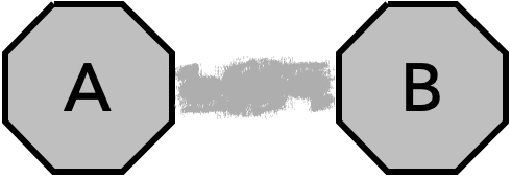
\includegraphics[width=\linewidth]{../../FIGURES/Bipartite-discovery.pdf}
  \caption{A Link yet to be discovered, or a flakey link that need to be repaired}
      \vspace{12pt}
\end{marginfigure}


\CELLs discover connections $\exists$xist on \emph{each} of their ports. For connections that  once existed (which may have been remembered from previously being powered up), we will find it \emph{impossible} to tell whether we are being woken up for the $1$st time, or the $N$th time*. \marginnote{*Sleeping Beauty paradox: Veritasium:  \href{https://youtu.be/XeSu9fBJ2sI?si=Nl70HKeFJT1Rlexb}{The Most Controversial Problem in Philosophy}}

Single Links are subject to \emph{partial} or \emph{total} failure. Although networks use the word  `partition', for example in the CAP Theorem\cite{CAP}, this concept is inappropriate except in the single \LINK case, when there's no communication with the other side; the  \emph{causal %Ref David Deutch
 universes**\marginnote{\emph{**Quantum Compatible Interpretation}}} are now isolated from each other.
 
\section{It takes Two to Tango, and Three to Party}

%\subsection{Alice, Bob, and Carol with 3 LINKs}

Because a single link between Alice and Bob can be causally disconnected by real-world, permanent or intermittent failures, an alternative: statistically--independent--failure--path is necessary, to recover from \LINK Failures.  % ADD MODAL LOGIC necessary, etc.
This is the heart of the  Æ \texttt{ATOMICITY} claim:   A local (one hop \LINK) \texttt{TRIANGLE}  is the minimum necessary.  See TRIANGLE Clocks later in this specification.

 \begin{marginfigure}
        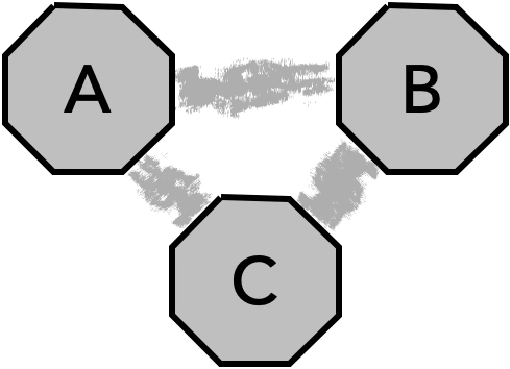
\includegraphics[width=\linewidth]{../../FIGURES/Tripartite-discovery.pdf}
  \caption{It takes three to party.  Links need an alternate path. This won't work over a Switched (Clos) Network.  
}
 %   \caption{A-B-C Flakey.pdf}
    \vspace{16pt}
\end{marginfigure}


\section{Alice  Bob,  and The role of Charlie}



%\subsection{\LINKs are Flakey}

 \begin{marginfigure}
      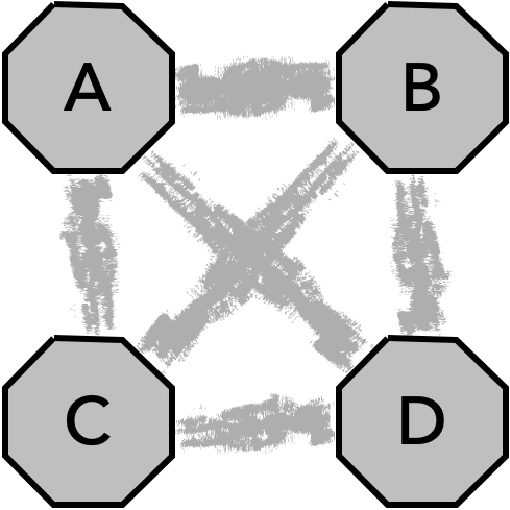
\includegraphics[width=\linewidth]{../../FIGURES/Quadpartite-discovery.pdf}
  \caption{2 x 2 =4  connected nodes with 6 flakey LINKs. Any one of which may be working in both directions: $\{11\}$, only one direction: $\{01\}$ or $\{10\}$, or \emph{not}-working in  \emph{both} directions: $\{11\}$. For 4 nodes, there are $\frac{(n(n-1)}{2} = 6$. With 4  \emph{reliability configurations} on each \LINK $\{00,01,10,11\}$ This gives us ONE correct (all links working correctly) and  $4^6-1 = 4095$ possible failure modes.}%\marginnote{permutations or combinations?} 
   \vspace{10pt}
\end{marginfigure}

\section{Graph Aware Determinism}

%In distributed systems, consensus protocols etc, it's easy to miss how varied network partitions can be. 

When treating the ``Network'' as an \emph{opaque cloud}, it's easy to underestimate how varied network partitions when link failures are 
asymmetrical:  A can see B, but B can't see A. In a 4 node setup, there are over 1295 potential partitions, and a flaky network can reproduce them all. % ref[ ]
From a distributed systems (event ordering in a cluster)  as an availability equation, we can easily overestimate how reliable they are, by 3 orders of magnitude.  

Link failures are invisible (hidden) in a Clos. They are 100\% Visible to us in a local graph of \emph{triangular} relationships.

And that's only the clean (binary) binary failures. Real system \emph{flakey} connections are much worse.

\subsection{Transactions need a coordinator\cite{Jim Gray}}

The Æthernet   protocol is designed to be exquisitely sensitive to packet loss and corruption We monitor, detect, diagnose link failures, and recover reversibly and automatically.


\newpage

\section{Fault Detection Model}

\marginnote{
Benefits include (i) Shorter packets and more effective use of bandwidth, (ii) more complete coverage of possible failure modes. (iii) Guarantees at least the first slice is perfect (matches what the transmitter knows they sent). }

AE-Links present two major differences to the conventional FEC thinking in today's Ethernet, which exploits the physics from 25Gb/s to 1.6Tb and beyond:

\begin{description}
\item [Perfect Information Transfer (PIF)] Æ-Links use Back-to-Back (B2B) Shannon Links, where the receiver returns the first 8-byte slice of each 64-Byte packet to the transmitter. This ``here is what I heard you say" ( Perfect Information Transfer (PIF)\cite{Paper from Garner}

\item [Epistricted Registers (EPI)] Borrowing from the Spekkens' toy model for quantum entanglement, we narrow down the possible entangled states to a vastly smaller set of possibilities, using the model described in Quantum Ethernet\cite{Quantum Ethernet}.
\end{description}



\section{Failure Model}

Consider a network of \(n\) nodes connected by undirected Ethernet
links.  Each link can be in one of four independent reliability
states,
\marginnote{
\[
\Sigma=\{00,01,10,11\},
\]}
where \(11\) means the link works in both directions, \(10\) or
\(01\) means it works in only one direction, and \(00\) means it
is broken in both directions.

\section{Link count}

Because every node may attach to at most eight neighbours (an
\emph{octavalent} mesh), the number of physical links is
\marginnote{
\[
L(n)=\min\!\bigl\{\tbinom{n}{2},\,4n\bigr\}
=
\begin{cases}
\binom{n}{2}, & n\le 9,\\[6pt]
4n,            & n\ge 9.
\end{cases}
\]}

\section{Reliability configurations}

Each link chooses a state from \(\Sigma\) independently, so the total
number of configurations is \(4^{\,L(n)}\).
Exactly one of these is fully healthy (all links in state \(11\)), hence
\[
\text{FailureModes}(n)=4^{\,L(n)}-1.
\]

\section{Enumerated results for \(2\le n\le20\)}

%\begin{table}[ht]
\begin{margintable}
\centering
\begin{tabular}{@{}rrr@{}}
\toprule
\(n\) & \(L(n)\) & Failure modes \(4^{\,L}-1\)\\
\midrule
 2 &  1 & 3\\
 3 &  3 & 63\\
 4 &  6 & 4\,095\\
 5 & 10 & 1\,048\,575\\
 6 & 15 & \(1.074\times10^{9}\)\\
 7 & 21 & \(4.398\times10^{12}\)\\
 8 & 28 & \(7.206\times10^{16}\)\\
% 9 & 36 & \(4.722\times10^{21}\)\\
%10 & 40 & \(1.209\times10^{24}\)\\
%11 & 44 & \(3.095\times10^{26}\)\\
%12 & 48 & \(7.923\times10^{28}\)\\
%13 & 52 & \(2.028\times10^{31}\)\\
%14 & 56 & \(5.192\times10^{33}\)\\
%15 & 60 & \(1.329\times10^{36}\)\\
%16 & 64 & \(3.403\times10^{38}\)\\
%17 & 68 & \(8.711\times10^{40}\)\\
%18 & 72 & \(2.230\times10^{43}\)\\
%19 & 76 & \(5.709\times10^{45}\)\\
%20 & 80 & \(1.462\times10^{48}\)\\
\bottomrule
\vspace{8pt}
\end{tabular}
\caption{Failure‑mode counts for an octavalent mesh with \(n\) nodes.}
\vspace{12pt}
\end{margintable}
%\end{table}

\section{Reliable, Deterministic Atomicity (RDA)}% without the Memory}


Reliable, Deterministic, Atomicity (RDA)\marginnote{All or nothing multicast token transfer across all observers.}  is achievable on an AE-LINK, as long as the Shannon Slots are continuously reconciled on both sides of the link by atomic token exchanges. However, a single link can break. This is why a 3rd party in the triangle (Carol  (causal arbiter) or Charlie (causal coordinator) is necessary.



%\documentclass[letterpaper]{tufte-handout}
%
%\usepackage{amsmath,amssymb,booktabs}
%
%\title{Counting Failure Modes for a 4‑Node Fully Connected Network}
%\author{}
%\date{\today}
%
%\begin{document}
%\maketitle

\section{Problem recap}

A fully connected network of \(n = 4\) nodes has
\[
L \;=\;\binom{4}{2} \;=\; 6
\]
undirected Ethernet links.

Each link independently assumes one of four reliability states
\[
\Sigma \;=\; \{\,00,\;01,\;10,\;11\,\}.
\]

\section{Correct failure‑mode count}

The total number of distinct network configurations is
\[
4^{\,L} \;=\; 4^{6} \;=\; 4096.
\]

Exactly one configuration represents the perfectly healthy network (all links working in both directions)
therefore the number of failure modes is
\[
4^{6} - 1 \;=\; 4095.
\]

\section{Where the earlier 1295 came from}

The earlier calculation reversed base and exponent,
using \(6^{4}\) instead of \(4^{6}\):
\[
6^{4} - 1 \;=\; 1295,
\]
which under‑counts the possibilities because it treats the
\emph{links} as the alphabet size and the \emph{state space} as the exponent.

\section{The Blast Radius of Link Failures in a 4-cell (4-node) system}

\begin{table}[h]
\centering
\begin{tabular}{@{}lll@{}}
\toprule
Method & Expression & Count \\
\midrule
Correct (states\(^\text{links}\)) & \(4^{6} - 1\) & 4095 \\
Earlier mis‑step (links\(^\text{states}\)) & \(6^{4} - 1\) & 1295 \\
\bottomrule
\end{tabular}
\caption{Failure‑mode counts for a 4‑node (6‑link) fully connected network.}
\end{table}

\newpage


\subsection{\LINK initialization}


\texttt{Alice} and \texttt{Bob} have no knowledge of each other prior to being powered up for the first time. They discover each other by sending and responding to \texttt{BEACON}s on each of their 8 ports $\{n,ne,de,se,ds,sw,dw,nw\}$. \texttt{BEACON}s are questions: ``is anyone there?'' They assume  neighbor \CELLs have SerDes' that can send \& receive @ 25Gb/s (defined by local clocks, in their frame of reference). Photon cavities (copper and fiber) are expected to be in a fixed frame of reference relative to the \texttt{SELF} \CELL.  Mobile entities may need to adjust this expectation based on the range of doppler shifts expected by \CELLs in motion, for example, in moving vehicles, \texttt{cars}, \texttt{planes}, and \texttt{spacecraft}.


Alice sends \texttt{BEACON}s with an exponential backoff: every $1\mu s$, $2 \mu s$, $4 \mu s$, 8 $\mu s$, etc. The  policy for a maximum interval  is determined by the environment, e.g. within a datacenter, one might wish to send  \texttt{BEACON}s every second, whether you need to or not.  This  represents a balance between infrastructure liveness and needless energy dissipation.

\section{Short-Range ANT (Local)  Scouting}

Once a link has been established, they are recorded in the local \texttt{knowledge} of the cell, and used as a baseline for future algorithmic and policy decisions. 

Immediately after establishing a reliable connection, \CELLs may emit \texttt{ANT-SCOUTS} to explore their local environment. These are ANT's, which obey an initial source routing algorithm, but when encountering a failed or disconnected port in another cell, respond with either clockwise, anticlockwse packet forwarding, which keeps the scout local, or \emph{random}, with a hopcount limit, which allows exploration further afield\marginnote{See ANT Specification for details}.

\section{Long-Range BEE (Global)  Scouting}

\CELLs may also emit \texttt{BEE-SCOUTS} to explore the extremities of their environment. These are BEE's which obey only one rule: proceed in the same direction as the radial port.   BEE's  emitted on the $n$ port may only go $n$.  BEEs emitted on the $se$ port may only go $se$. Until they encounter a disconnected port, whereupon they execute a return path algorithm, accumulating information at each \CELL and returning it to the root.\marginnote{See BEE specification for details}



\newpage
\section{ANT Specification: Triangle Packet Clocks in $3 \times 3$ Tiles}
 \begin{marginfigure}
        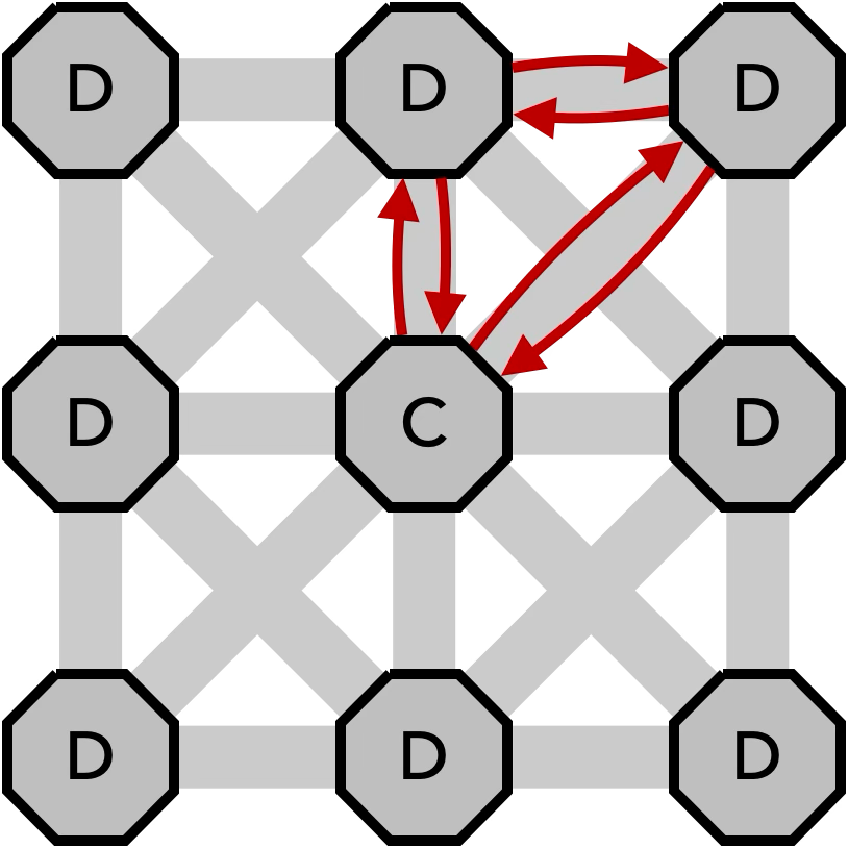
\includegraphics[width=\linewidth]{../../FIGURES/Triangle-clock.pdf} % Trim is l b r t
  \caption{Race-Free Triangle Token}
    \vspace{10pt}
\end{marginfigure}

Packet clocks are initiated by the coordinator, on any of it's active links.  The ANT (source routing) algorithm goes out on any port, and are programmed to turn left or right at the first available active port.  The convention is turning right makes it go clockwise, and turning left makes it go antilockwise, but this is an artificial distinction. As with real ants, they can get lost, and never find their way back to the nest, and they die (or return to the nest by inverting their source routing paths). This ``limited range'', is part of the Security mechanism. 

\section{ANT Specification: Race-Free Packet Clocks in $3 \times 3$ Tiles}
 \begin{marginfigure}
        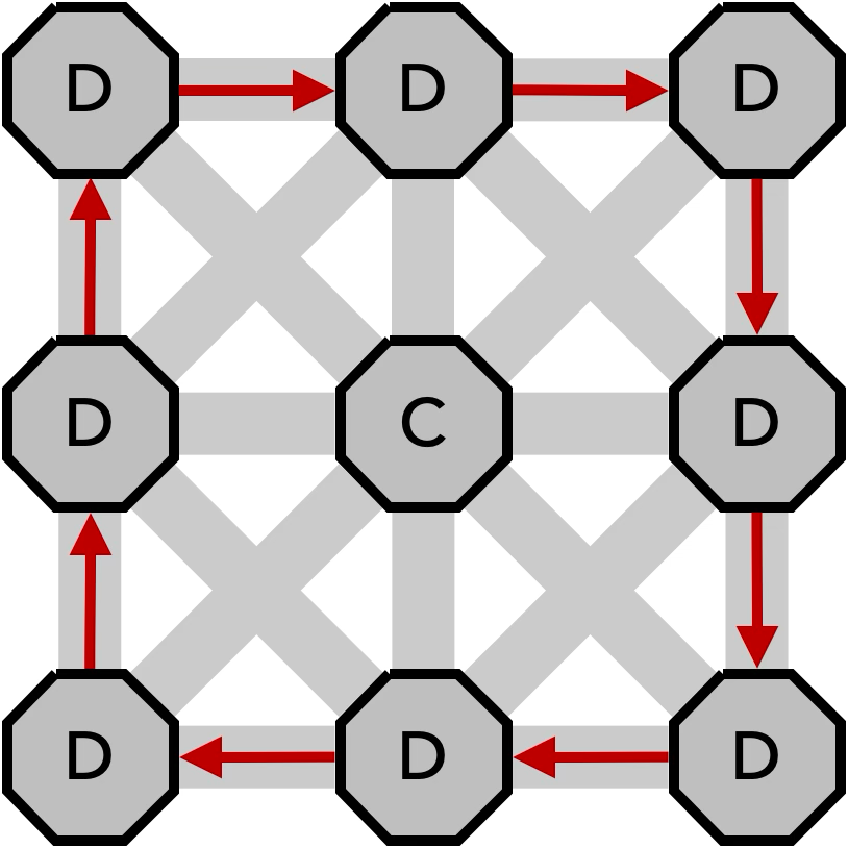
\includegraphics[width=\linewidth,trim=0mm 0mm 0mm 0mm, clip]{../../FIGURES/3x3-clockwise.pdf} % Trim is l b r t
  \caption{Square Race-Free 1-hop Clock}
    \vspace{10pt}
\end{marginfigure}




 \begin{marginfigure}
        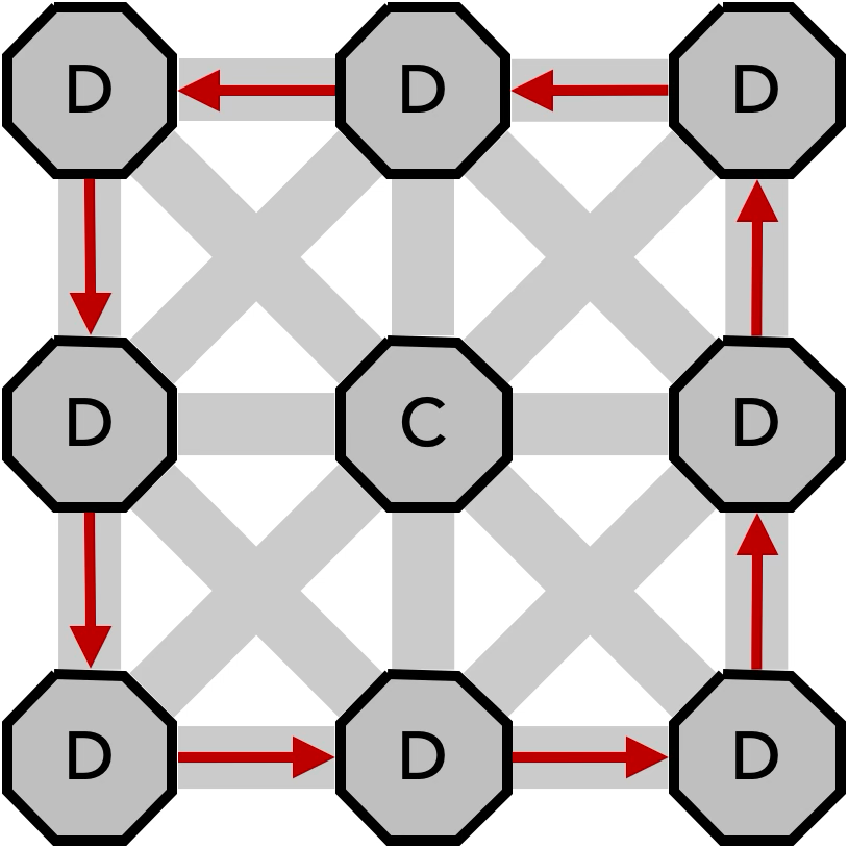
\includegraphics[width=\linewidth,trim=0mm 0mm 0mm 0mm, clip]{../../FIGURES/3x3-anticlockwise.pdf} % Trim is l b r t
  \caption{Race-Free Anticlockwise }
    \vspace{10pt}
\end{marginfigure}

Once the cell has discovered it's local environment, it may establish packet clocks. These are ANTs, which go out with a pre-defined pattern, to return events the cell on a \emph{periodic} basis.  Because there is no \emph{background} of time, this system will create events, which are guaranteed to occur without race conditions, but will catastrophically fail if there are an broken links around the circuit.

 \begin{marginfigure}
        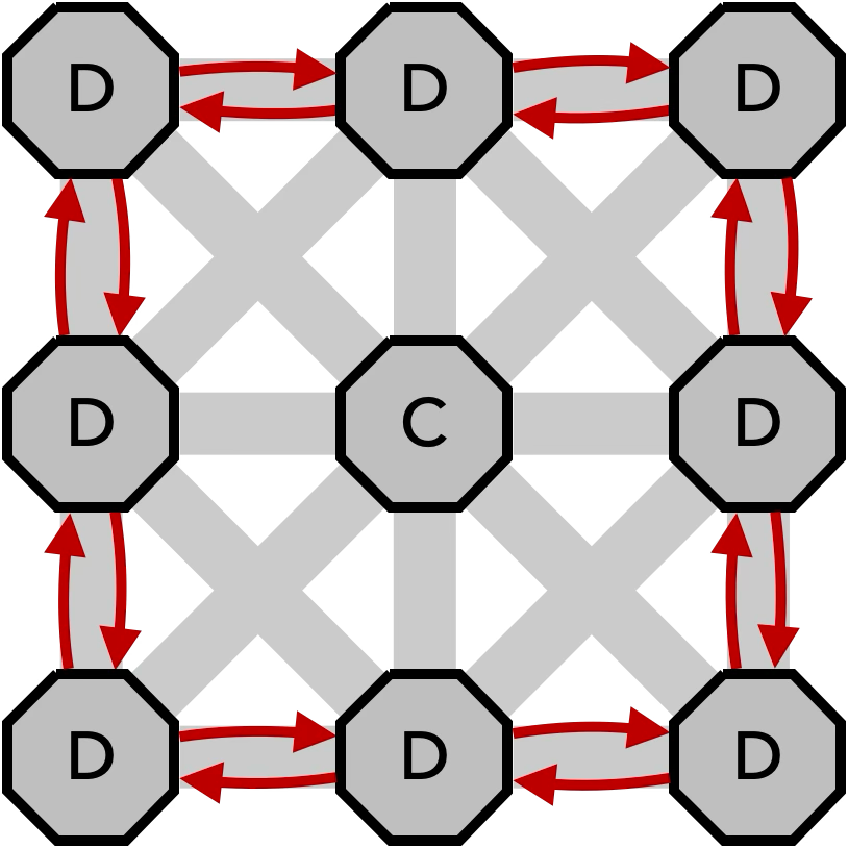
\includegraphics[width=\linewidth,trim=0mm 0mm 0mm 0mm, clip]{../../FIGURES/3x3-bothways.pdf} % Trim is l b r t
  \caption{2 Circulating Race-free tokens }
    \vspace{10pt}
\end{marginfigure}

Packets clocks may be initiated around  the closest (one-hop) cell tiles, next closest (two-hop) tiles, furthest (three-hop) tiles. Atomicity 

% FROM Spec Document SPREADSHEET-GVM copy.numbers
\subsection{ANT Specification Building a Compass Clock}
8 physical ports per cell. 
Inactive ports may be:
\begin{itemize}
\item Failed (out of service)
\item Standby, ready to go
\item Off, saving energy
\end{itemize}

\subsection{ANT Specification: Counter Circulating Race-Free ANTS}

C (Carol, Charlie, Coordinator, Chief) may initiate clockwise, counter-clockwise, and/or both at once. Each is exploring the health of the connectivity local to the center cell. This is what ANT Algorithms (source routed, or random) tokens. 



Ports at edge of mesh connected back to same cell on a different port to traverse routing table 2nd time to create  virtual cut-through torus.

If the ANT gets blocked, and either runs out of hopcout resource, it does `reverse path forwarding' back to the C CELL. and reports what it finds. It can either carry all its state in the packet, or (ror BEEs), clean up on its way and erase its footprints in the CELLs it visited.



%\section{Packet Clocks}

\newpage

\subsection{7 x 7 Nodes Packet Clock}

 \begin{marginfigure}
        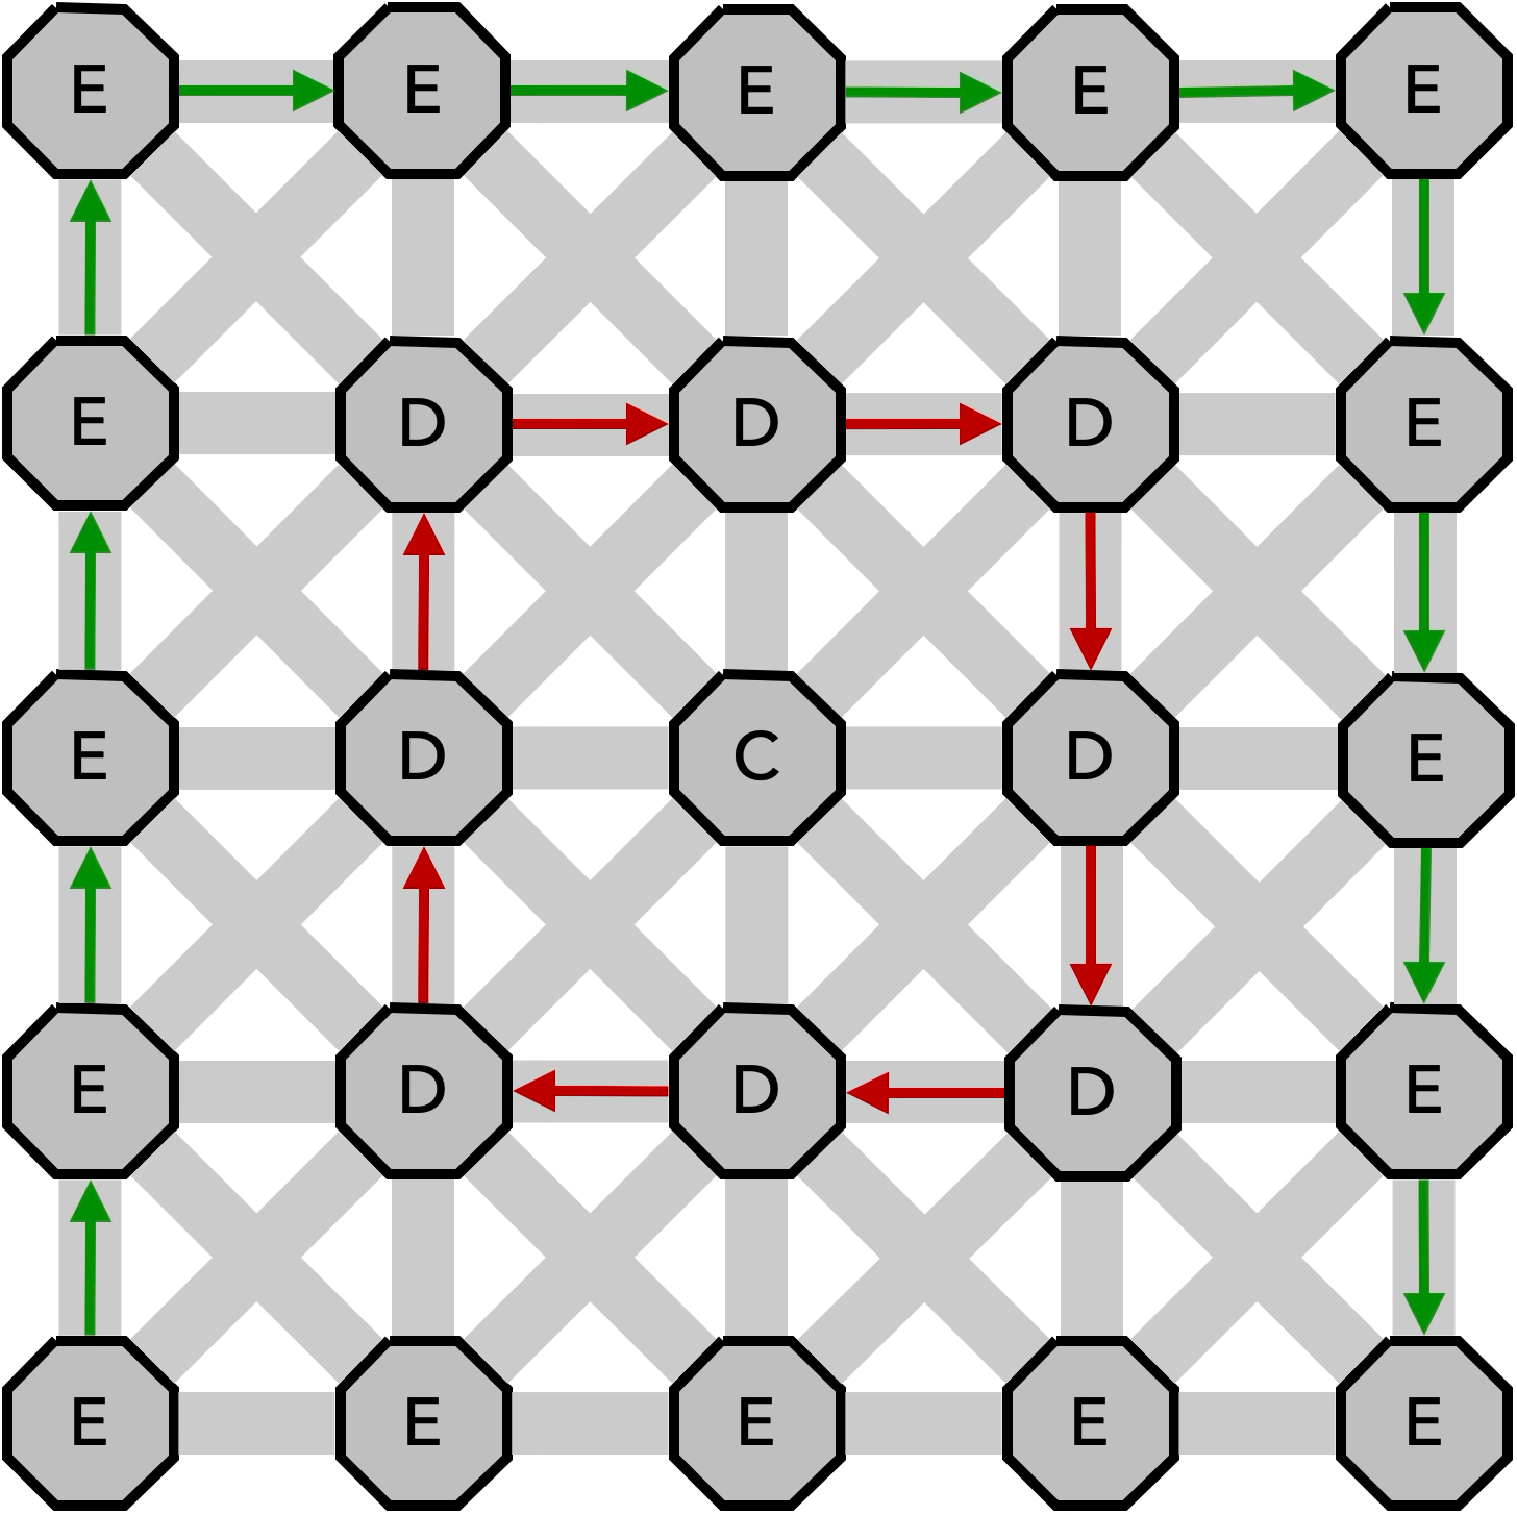
\includegraphics[width=\linewidth,trim=0mm 0mm 0mm 0mm, clip]{../../FIGURES/5x5-clock.pdf} % Trim is l b r t
  \caption{Green Packet Rateless Clock}
    \vspace{20pt}
\end{marginfigure}

\section{Beyond Packet Clocks}

Packet clocks don't scale (they are not intended to). Instead, they provide circulating logical loops \cite{Logical Clocks}.  The local system policy will establish the radius limit for local exploration. Everything beyond that is in the domain of the BEE scouts .

Packet clocks can circulate at any physical hop distance. The one-hop agents are described above.  The two figures on the right show an example of an ANT which goes two hops, or three hops, before the ANT turns left or right.  This give a CELL the opportunity to explore larger hop distances from the coordinator

\section{Packet Clocks in Larger Tiles}

 \begin{marginfigure}
        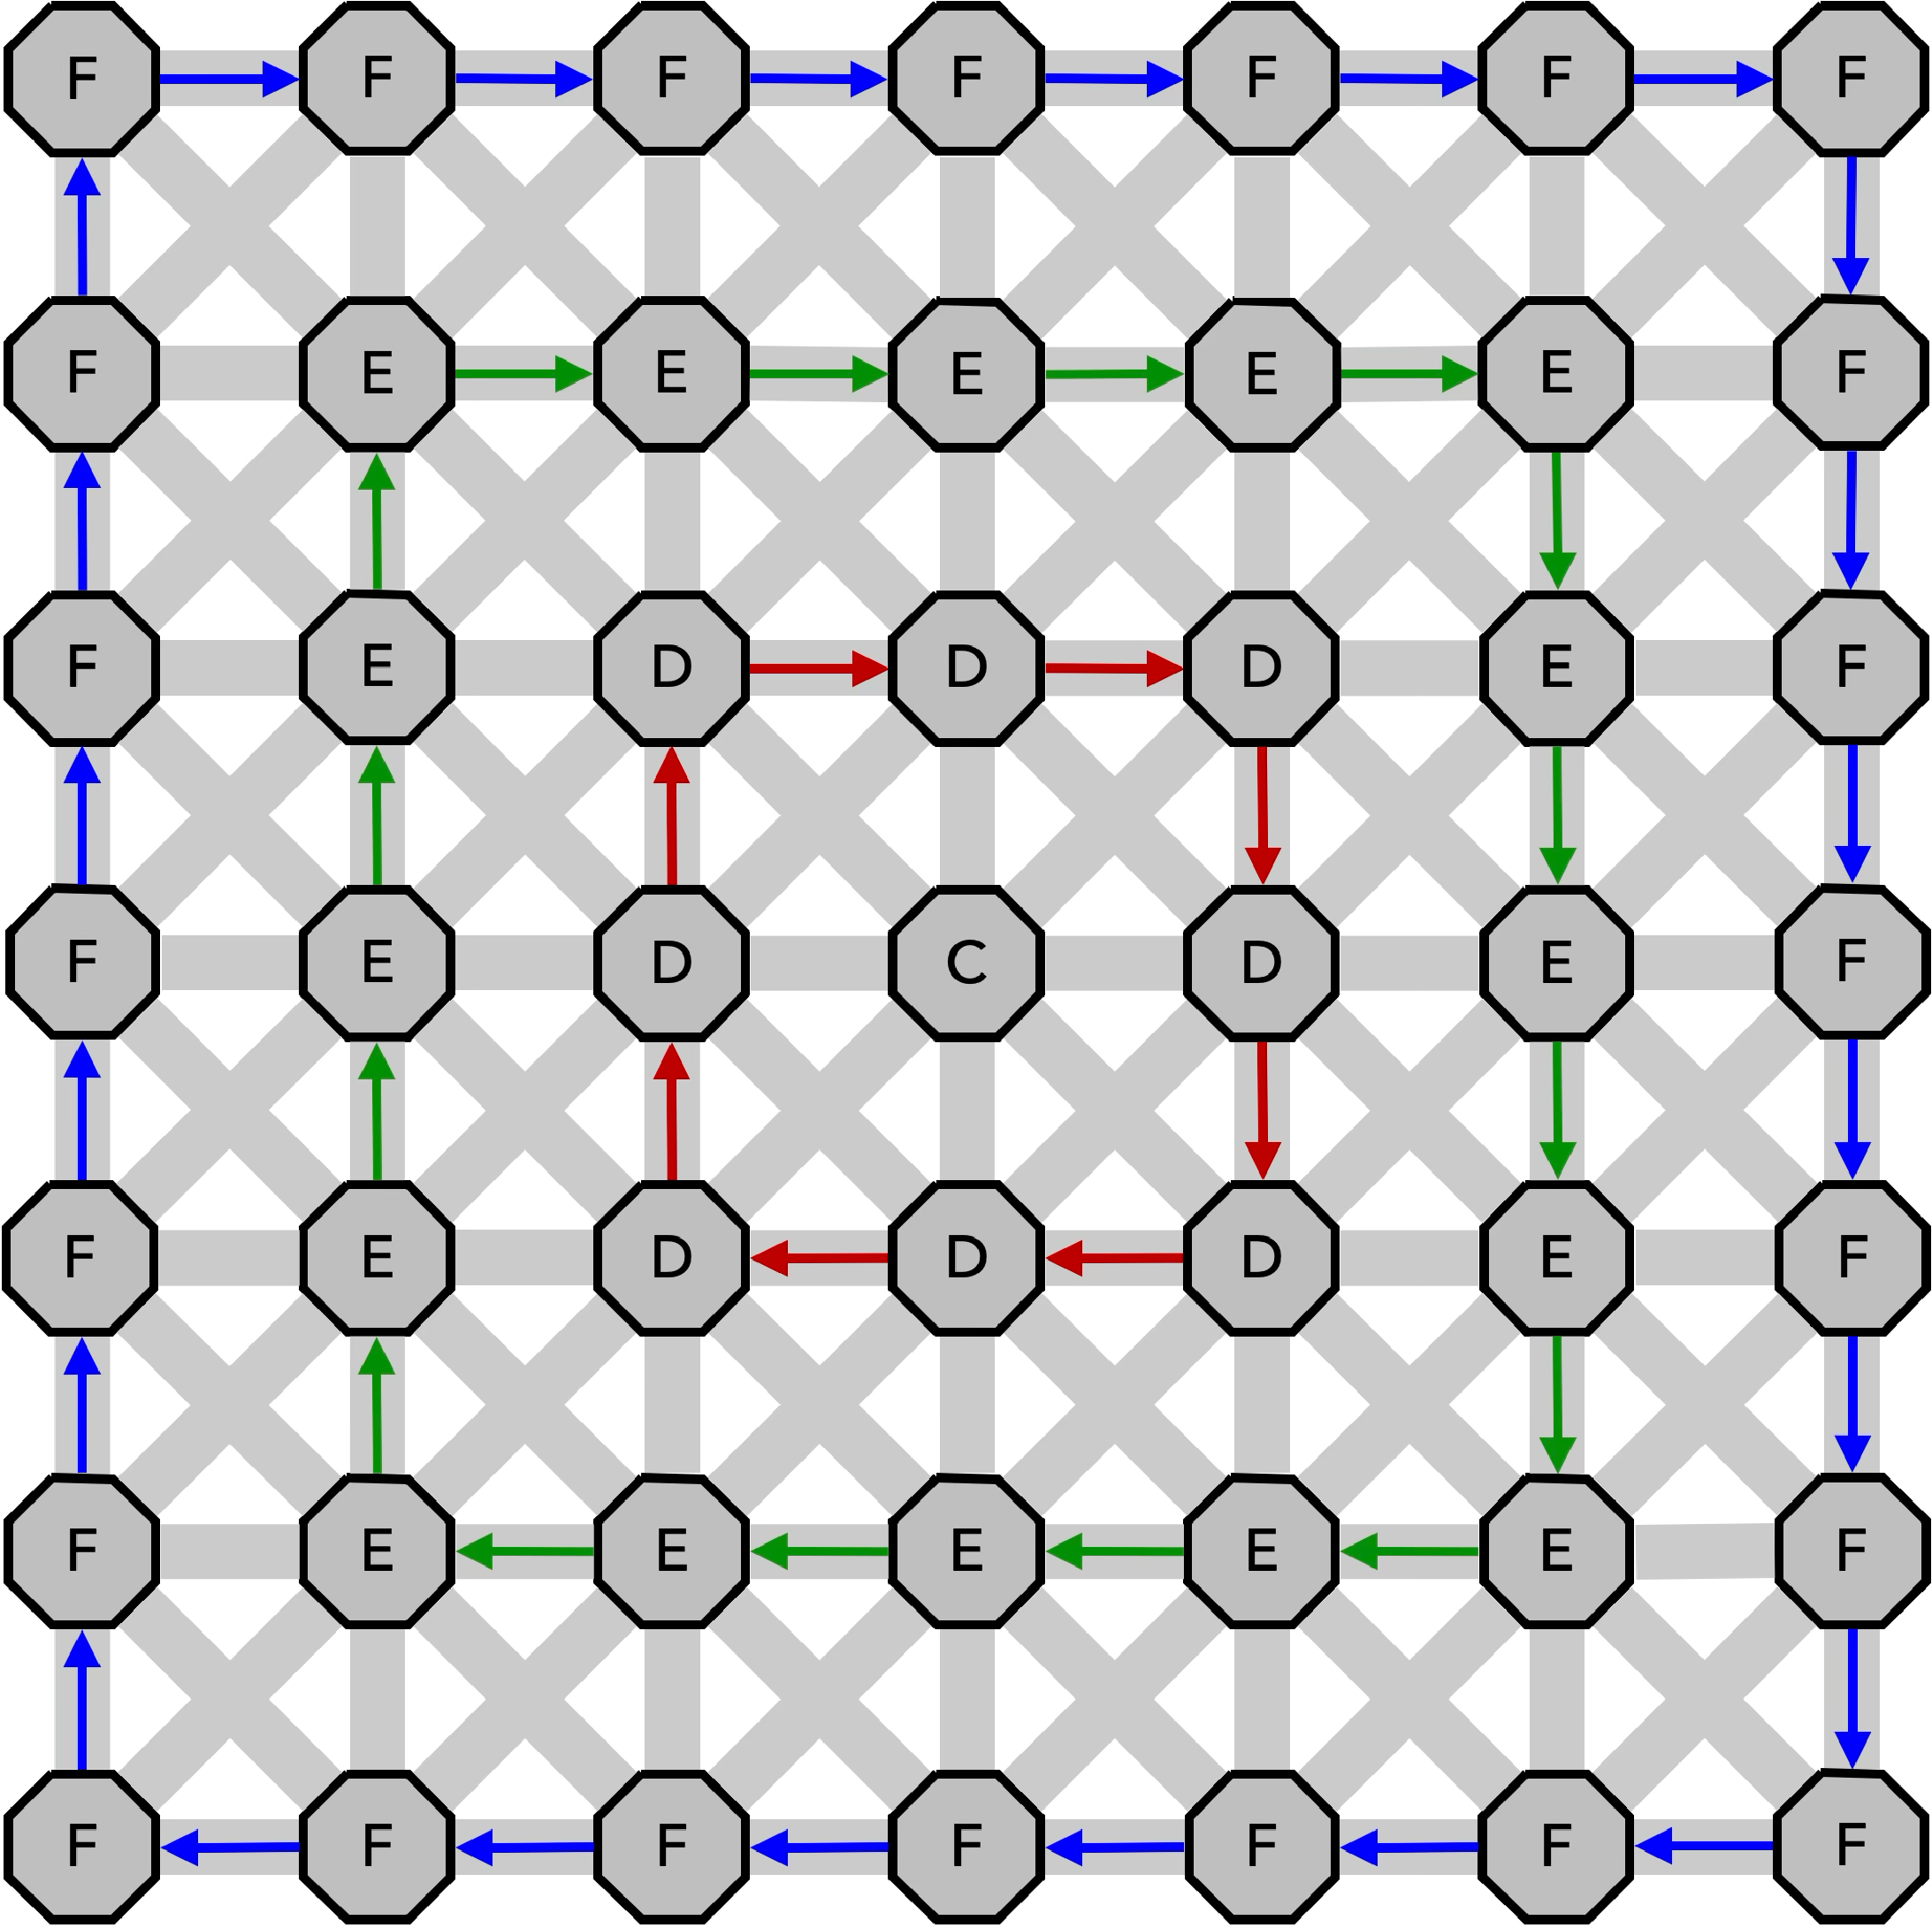
\includegraphics[width=\linewidth,trim=0mm 0mm 0mm 0mm, clip]{../../FIGURES/7x7-clock.pdf} % Trim is l b r t
  \caption{3rd-hop circular packet clocks. Blue Links Complete}
    \vspace{20pt}
\end{marginfigure}

\subsection{BEE scouts}

BEE Scouts explore the boundaries of their environment.  The are emitted by the Coordinator, and travel as far as they can in ONE direction, \texttt{\{dn,ne,de, se, ds, sw, dw, nw\}}, and then \emph{return on the reciprocal path (Compass-Point vector direction)} to inform the hive (root) what they discovered, so the root can build it's model of the topology, and Edge resources to perform their function. 

\subsection{N x N Nodes Packet Search Rays (BEEs)}

BEEs  are radial distance scouting agents. Single packets that go in only one direction, and when they reach the end (extremities of the Cellular interconnect) they execute a reverse path forwarding algorithm, collecting knowledge on their way, delivering this knowledge back to the root, whose agent  uses the returned information to build it's model of it's topology and available resources to offer `services' to the applications.

These don't have to be square, or rectangular. BEE algorithms work on any arbitrary Topology.

 \begin{marginfigure}
        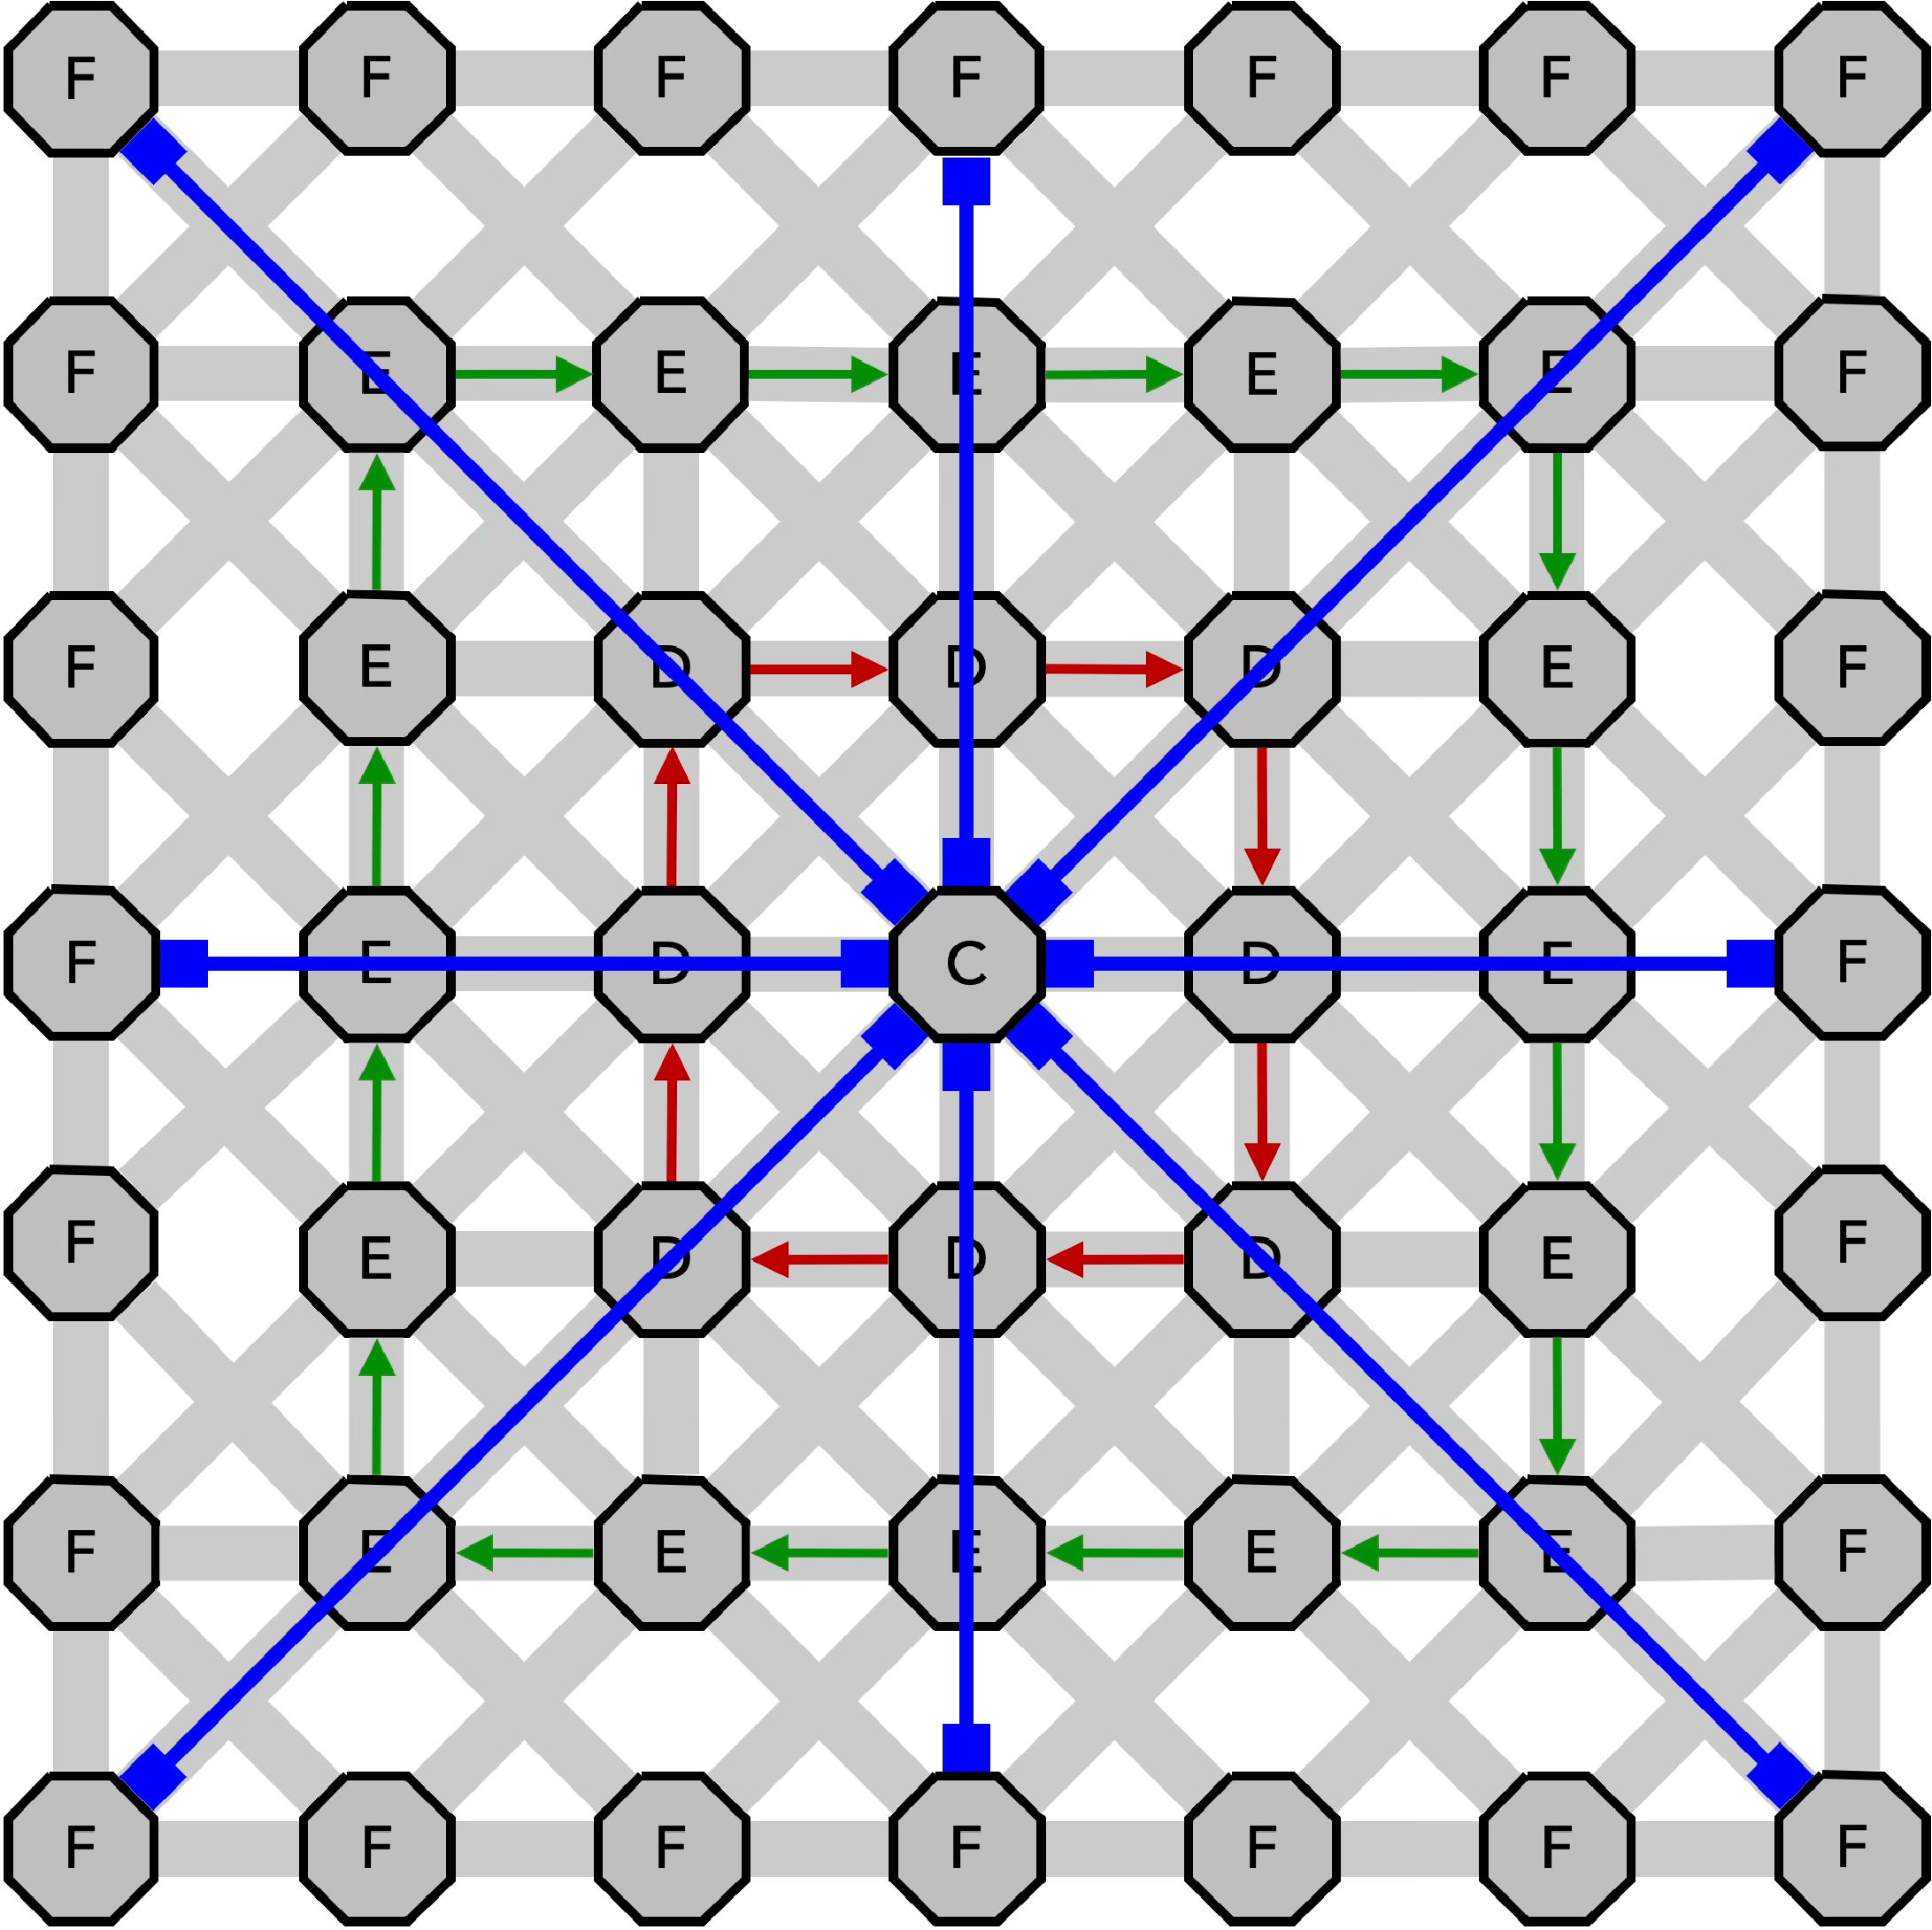
\includegraphics[width=\linewidth,trim=0mm 0mm 0mm 0mm, clip]{../../FIGURES/7x7-rays.pdf} % Trim is l b r t
  \caption{BEE Algorithms explore beyond ANT algorithms}
    \vspace{20pt}
\end{marginfigure}

Radial (Ray) source-routed scouts have two parameters (a) which port they go out on, and continue indefinitely until they reach a boundary (or exhaust their hop count resource). And then they return along exactly the same path, accumulating knowledge of the CELLS on their way (e.g. properties of the cell, do they have a CPU, a GPU, an IPU, or QPU?).  Most Bees make it back home to the nest (C) but it is also possible for a failure to occur between the outbound BEE and the homebound BEE. In which case the packet try's to make it's way to `Lost and Found', the control structures identified by the Coordinator to provide GEV notification of failures.  Lost and Found is most likely to be discovered by the one or more of the BEEs. Edge nodes (on the corners of the interconnect), will always be able to `find' Lost and Found (and other external control paths controlled by monitoring or configuration LOGICAL Administrator Agentss ) with a `due north or south'  \texttt{dn,ds}, `due-east or west' \texttt{de,dw} BEE Scout. 


 


\section{Distributed Systems}


\section{Set Reconciliation of Shannon Slots}

The first claim is that a finite and enumerable number of  `slots' exist on both sides of the LINK. In conventional Ethernet, once these slots are exhausted (with for example, a timeout and retry, the XPU CELLS (SmartNICs) on both sides of the LINK must evict (erase) the information on one side and then the other. This `loss of Koherence' is the central problem of Distributed Systems.  From an information theoretic (Back to Back Shannon channel) perspective, this precipitates a `smash and restart (SAR) of the Shannon Information --  the loss of `pairing' of information. This is described in more detail in the specification of back-to-back Shannon Pairs.

Timeouts and Retries are the root of all evil.  Once a Timeout Storm occurs, in a switched network, the distributed systems in the Host processor are all broken. Unless RELIABILITY (maintenance of Shannon Link Pairing),  the `global' illusion of event ordering in distributed systems will be lost, and corruption will occur.  This is why queue-pairs work in Infiniband/RDMA. This is why information pairing is essential, in Tandem's Process Pairs, and RDMA's Queue pairs.

The whole point of this specification is to engineer a solution, where Shannon-pairing is never lost, but if it is, a TRIANGLE healing occurs locally, without the need to depend on a switched or router to discover and  `reconverge' their routing tables, to re-establish the point to point connections over a different paths in the network.  

The main mechanism to do this is to make the Æthernet Link maintain Koherence, and when loss occurs, a 3rd party (The Triangle relationship) can recover with local information only. This makes XPU/SmartNICs, where the recovery algorithms (healing the tree) occur locally, instead of waiting for the switched or routed packets (in a separate switched network.

The original Ethernet was unreliable. This was a mistake. Infiniband already proved this, and succeeded both in the trust system archicitcts have in the far greater. The unique contributions of this specification is to go (far) beyond Infiniband's discovery, and recognize the fundamental simplifications and benefits that Infiniband (and Token Ring,  Fibrechannel, and Sonet), in creating `Race-Free' protocols, where distributed systems can guarantee, not just the `ordering of events', but the guarantee of recovery of transactional loss in when failures occur in the middle of, say, a 2 Phase Commit. 

Æthernet (Atomic Ethernet) guarantees that Shannon Pairing is never lost, and if a link breaks, that the Coordinator (Charlie, Carol, Chief) can recover with TRIANGLE Relationships, far faster than any protocol stack in the host processor, or in the RMDA message relationships, but then add, on top of this a true `atomic' relationship between CELLS (nodes) in a distributed system.

The original Ethernet [ref] was designed around a notion of slots. These were `time slots' on an imaginary timeline that each node on the Ethernet Cable, could manage in a half-Duplex way.  The new notion is to replace this with circulating tokens, where each slice is independently acknowledged, providing a guarantee of delivery to the NEXT hop in the network.

This is achieved with 1PC (one phase commit), where each Ethernet Packet (eight slices) are fully acknowledged in each link. The generalization of this is to explicitly manage Shannon slots (data structures on each side of the link) to maintain Koherence, even when the link fails (in one direction, the other direction, or in both directions at once).

This can be done (as in Fibrechannel)  by arranging the `interaction protocol' to guarantee the pairing of events, and not resort to Timeout and Retry (TAR), which causes cascade failures in networks, both large and small.

This is achieved with the Link Protocol employing the Alternating Bit protocol, and adding the Bill Lynch ABP reconciliation, with two or more bits instead of the individual 1 bit of alternation, which required a round trip to guarantee Shannon Slot Pairing.



\section{FAQ}

Q1 (Alan) What problem are you addressing in the scouting writeup?  If it’s discovering routes, it’s not clear to me that ant or bees or even both together do full discovery of the network.  In what way are they better than the flooding algorithm I used?

A1 This is how to achieve `Scale-Independence' We eliminate the need for   every node  to do a `full discovery' of the network, which is what a flooding algorithm would do.  ANTs and BEEs explicitly do not do ``Global" routing. This is an extra way to limit the size of the secure enclave, and not have it able to connect to the outside world.  


\end{document}